\documentclass[11pt]{article}
\usepackage{amsmath}
\usepackage{amssymb}
\usepackage{graphicx}
\usepackage{tabularx}
\usepackage{fancyhdr}
\usepackage{lastpage}

% Page layout
\usepackage[top=1in, bottom=1in, left=1in, right=1in]{geometry}

% Header and footer
\pagestyle{fancy}
\fancyhf{}
\rfoot{Page \thepage}
\renewcommand{\headrulewidth}{0pt}

% Modified Question command with left-aligned number
\newcommand{\questiona}[2]{
    \noindent\textbf{Q#2.} #1 \hfill \textbf{[1 Mark]}
}

\newcommand{\questionb}[2]{
    \noindent\textbf{Q#2.} #1 \hfill \textbf{[2 Marks]}
}

\begin{document}

% Title section with horizontal line
\begin{center}
    \Large\textbf{GATE 2017 - Petroleum Engineering (PE)} \\
    \large\textbf{General Aptitude and Technical Questions} \\
    \rule{\textwidth}{0.5pt} % Horizontal line below heading
\end{center}

\vspace{0.5cm}

% General Aptitude Section
\section*{General Aptitude}

\questiona{The ninth and the tenth of this month are Monday and Tuesday \_\_\_\_\_.}{1}
\begin{enumerate}
    \item[(A)] figuratively  
    \item[(B)] retrospectively  
    \item[(C)] respectively  
    \item[(D)] rightfully  
\end{enumerate}
\vspace{0.5cm}

\questiona{It is \_\_\_\_\_ to read this year's textbook \_\_\_\_\_ the last year's.}{2}
\begin{enumerate}
    \item[(A)] easier, than  
    \item[(B)] most easy, than  
    \item[(C)] easier, from  
    \item[(D)] easiest, from  
\end{enumerate}
\vspace{0.5cm}

\questiona{A rule states that in order to drink beer, one must be over 18 years old. In a bar, there are 4 people. P is 16 years old, Q is 25 years old, R is drinking milkshake and S is drinking a beer. What must be checked to ensure that the rule is being followed?}{3}
\begin{enumerate}
    \item[(A)] Only P's drink  
    \item[(B)] Only P's drink and S's age  
    \item[(C)] Only S's age  
    \item[(D)] Only P's drink, Q's drink and S's age  
\end{enumerate}
\vspace{0.5cm}

\questiona{Fatima starts from point P, goes North for 3 km, and then East for 4 km to reach point Q. She then turns to face point P and goes 15 km in that direction. She then goes North for 6 km. How far is she from point P, and in which direction should she go to reach point P?}{4}
\begin{enumerate}
    \item[(A)] 8 km, East  
    \item[(B)] 12 km, North  
    \item[(C)] 6 km, East  
    \item[(D)] 10 km, North  
\end{enumerate}
\vspace{0.5cm}

\questiona{500 students are taking one or more courses out of Chemistry, Physics, and Mathematics. Registration records indicate course enrolment as follows: Chemistry (329), Physics (186), Mathematics (295), Chemistry and Physics (83), Chemistry and Mathematics (217), and Physics and Mathematics (63). How many students are taking all 3 subjects?}{5}
\begin{enumerate}
    \item[(A)] 37  
    \item[(B)] 43  
    \item[(C)] 47  
    \item[(D)] 53  
\end{enumerate}
\vspace{0.5cm}

\questionb{"If you are looking for a history of India, or for an account of the rise and fall of the British Raj, or for the reason of the cleaving of the subcontinent into two mutually antagonistic parts and the effects this mutilation will have in the respective sections, and ultimately on Asia, you will not find it in these pages; for though I have spent a lifetime in the country, I lived too near the seat of events, and was too intimately associated with the actors, to get the perspective needed for the impartial recording of these matters." Which of the following statements best reflects the author's opinion?}{6}
\begin{enumerate}
    \item[(A)] An intimate association does not allow for the necessary perspective.
    \item[(B)] Matters are recorded with an impartial perspective.
    \item[(C)] An intimate association offers an impartial perspective.
    \item[(D)] Actors are typically associated with the impartial recording of matters.
\end{enumerate}
\vspace{0.5cm}

\questionb{Each of P, Q, R, S, W, X, Y and Z has been married at most once. X and Y are married and have two children P and Q. Z is the grandfather of the daughter S of P. Further, Z and W are married and are parents of R. Which one of the following must necessarily be FALSE?}{7}
\begin{enumerate}
    \item[(A)] X is the mother-in-law of R  
    \item[(B)] P and R are not married to each other  
    \item[(C)] P is a son of X and Y  
    \item[(D)] Q cannot be married to R  
\end{enumerate}
\vspace{0.5cm}

\questionb{1200 men and 500 women can build a bridge in 2 weeks. 900 men and 250 women will take 3 weeks to build the same bridge. How many men will be needed to build the bridge in one week?}{8}
\begin{enumerate}
    \item[(A)] 3000  
    \item[(B)] 3300  
    \item[(C)] 3600  
    \item[(D)] 3900  
\end{enumerate}
\vspace{0.5cm}

\questionb{The number of 3-digit numbers such that the digit 1 is never to the immediate right of 2 is}{9}
\begin{enumerate}
    \item[(A)] 781  
    \item[(B)] 791  
    \item[(C)] 881  
    \item[(D)] 891  
\end{enumerate}
\vspace{0.5cm}

\questionb{A contour line joins locations having the same height above the mean sea level. The following is a contour plot of a geographical region. Contour lines are shown at 25 m intervals in this plot.}{10}
\begin{center}
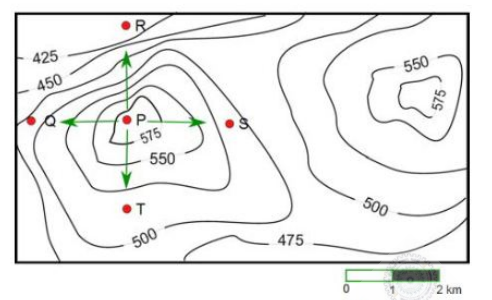
\includegraphics[width=0.5\textwidth]{figures/10.png}
\end{center}
Which of the following is the steepest path leaving from P?
\begin{enumerate}
    \item[(A)] P to Q  
    \item[(B)] P to R  
    \item[(C)] P to S  
    \item[(D)] P to T  
\end{enumerate}
\vspace{0.5cm}

% Technical Section
\section*{Technical Section}

\questiona{If a vector \( v \) has components \( v_x = 1, v_y = 2, v_z = 3 \), then its magnitude is \_\_\_\_\_. (write answer with two decimal places)}{1}
\vspace{0.5cm}

\questiona{The value of \(\lim_{x \to 0} \frac{(2 + x)^4 - 16}{x}\) is \_\_\_\_\_.}{2}
\vspace{0.5cm}

\questiona{If \(\frac{d^2 y}{dx^2} + f(x, y) = 0\) is to be solved using the conditions \(y(0) = a\) and \(y(1) = b\), which of the following numerical method(s) can be used?}{3}
\begin{enumerate}
    \item[(A)] Euler with shooting method  
    \item[(B)] Euler without shooting method  
    \item[(C)] \(4^{\text{th}}\) order Runge-Kutta with shooting method  
    \item[(D)] Both (A) and (C)  
\end{enumerate}
\vspace{0.5cm}

\questiona{The numerical method used to find the root of a non-linear algebraic equation, that converges quadratically, is:}{4}
\begin{enumerate}
    \item[(A)] Bisection method.  
    \item[(B)] Regula-falsi method (Method of False Position).  
    \item[(C)] Newton-Raphson method.  
    \item[(D)] None of above.  
\end{enumerate}
\vspace{0.5cm}

\questiona{Which one of the following curves shows a typical behavior of the producing gas oil ratio (GOR) with time for a reservoir under solution gas drive?}{5}
\begin{center}
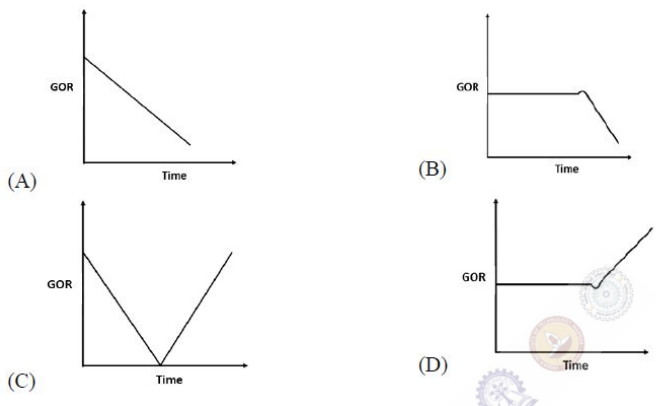
\includegraphics[width=0.8\textwidth]{figures/5.png}
\end{center}
\vspace{0.5cm}

\questiona{A student has written following possible causes of lost circulation during a drilling operation:}{6}
\begin{itemize}
    \item i. High salinity in the reservoir  
    \item ii. Fracture in the reservoir  
    \item iii. A fault encountered during drilling  
    \item iv. Low viscosity of the reservoir fluid  
\end{itemize}
Which of the above statements are correct?  
\begin{enumerate}
    \item[(A)] i, iv  
    \item[(B)] ii, iii  
    \item[(C)] i, iii  
    \item[(D)] ii, iv  
\end{enumerate}
\vspace{0.5cm}

\questiona{For water depth less than 8 m, which one of the following drilling vessels is the most suitable and economical?}{7}
\begin{enumerate}
    \item[(A)] Semi-submersible rig  
    \item[(B)] Jack-up rig  
    \item[(C)] Drilling barges  
    \item[(D)] Drill ship  
\end{enumerate}
\vspace{0.5cm}

\questiona{Which one of the following statements is correct for pseudo-steady state condition in a confined reservoir?}{8}
\begin{enumerate}
    \item[(A)] The pressure decline stops in the reservoir.  
    \item[(B)] The pressure declines at the same rate across the reservoir.  
    \item[(C)] The boundary pressure does not change.  
    \item[(D)] The pressure starts increasing in the reservoir.  
\end{enumerate}
\vspace{0.5cm}

\questiona{The roots of the equation \(\frac{d^3 y}{dx^3} - 6 \frac{d^2 y}{dx^2} + 11 \frac{dy}{dx} - 6y = 0\) are:}{9}
\begin{enumerate}
    \item[(A)] 1,1,2  
    \item[(B)] 1,2,3  
    \item[(C)] 1,3,4  
    \item[(D)] 1,2,4  
\end{enumerate}
\vspace{0.5cm}

\questiona{The \(^\circ\)API of a crude oil of density 950 kg/m\(^3\) is \_\_\_\_\_. (write answer with two decimal places)}{10}
\vspace{0.5cm}

\questiona{The differential equation \(2xy dx + (1 + x^2) dy = 0\), in which \(x\) is an independent variable and \(y\) is the dependent variable, is:}{11}
\begin{enumerate}
    \item[(A)] an ordinary differential equation of second order.  
    \item[(B)] a first order nonlinear differential equation.  
    \item[(C)] an exact differential equation.  
    \item[(D)] a partial differential equation.  
\end{enumerate}
\vspace{0.5cm}

\questiona{For the two matrices \( X = \begin{bmatrix} 1 & 2 & 3 \\ 4 & 5 & 6 \end{bmatrix}, Y = \begin{bmatrix} 7 & 0 \\ 8 & -1 \end{bmatrix} \), the product \( YX \) will be:}{12}
\begin{enumerate}
    \item[(A)] \( YX = \begin{bmatrix} 7 & 14 & 21 \\ 4 & 11 & 18 \end{bmatrix} \)  
    \item[(B)] \( YX = \begin{bmatrix} 4 & 11 & 18 \\ 7 & 14 & 21 \end{bmatrix} \)  
    \item[(C)] \( YX = \begin{bmatrix} 7 & 14 & 18 \\ 14 & 11 & 21 \end{bmatrix} \)  
    \item[(D)] \( YX = \begin{bmatrix} 7 & 14 & 21 \\ 18 & 5 & 6 \end{bmatrix} \)  
\end{enumerate}
\vspace{0.5cm}

\questiona{As per the Bharat IV norms, the maximum permissible limit of sulfur in diesel in ppm is:}{13}
\begin{enumerate}
    \item[(A)] 10  
    \item[(B)] 50  
    \item[(C)] 100  
    \item[(D)] 500  
\end{enumerate}
\vspace{0.5cm}

\questiona{The amount of methane gas evolved at 0°C and 1 atm from the dissociation of 1 m\(^3\) of methane gas hydrate, is approximately:}{14}
\begin{enumerate}
    \item[(A)] equal to the volume of gas hydrate.  
    \item[(B)] 10 times the volume of gas hydrate.  
    \item[(C)] 160 times the volume of gas hydrates.  
    \item[(D)] 300 times the volume of gas hydrates.  
\end{enumerate}
\vspace{0.5cm}

\questiona{For a centrifugal pump, the head developed by the pump is proportional to the:}{15}
\begin{enumerate}
    \item[(A)] speed of the impeller rotation.  
    \item[(B)] square of speed of the impeller rotation.  
    \item[(C)] cubic power of speed of the impeller rotation.  
    \item[(D)] square root of speed of the impeller rotation.  
\end{enumerate}
\vspace{0.5cm}

\questiona{Which of these is a must for petroleum generation and accumulation?}{16}
\begin{enumerate}
    \item[(A)] Source rocks  
    \item[(B)] Porous reservoir rocks  
    \item[(C)] Impermeable cap rocks  
    \item[(D)] All of the above  
\end{enumerate}
\vspace{0.5cm}

\questiona{The problem of viscous fingering is encountered when:}{17}
\begin{enumerate}
    \item[(A)] a low viscosity fluid is injected in a high viscosity fluid.  
    \item[(B)] a high viscosity fluid is injected in a low viscosity fluid.  
    \item[(C)] a fluid of equal viscosity but lower density is injected in a fluid of higher density.  
    \item[(D)] none of the above.  
\end{enumerate}
\vspace{0.5cm}

\questiona{Which of these is \textbf{NOT} a sedimentary rock?}{18}
\begin{enumerate}
    \item[(A)] Shale  
    \item[(B)] Sandstone  
    \item[(C)] Carbonate  
    \item[(D)] None of the above  
\end{enumerate}
\vspace{0.5cm}

\questiona{The \textbf{unbiased} sample variance for the set of numbers: \( S = \{40, 45, 50, 55, 60\} \) is \_\_\_\_\_. (write answer with one decimal place)}{19}
\vspace{0.5cm}

\questiona{If \( 5x + 2jy - ix + 7y = 2 + 3i \), where \( i = \sqrt{-1} \), the values of two real numbers \((x, y)\) are, respectively:}{20}
\begin{enumerate}
    \item[(A)] (-1, 1)  
    \item[(B)] (1, -1)  
    \item[(C)] (1, 1)  
    \item[(D)] (-1, -1)  
\end{enumerate}
\vspace{0.5cm}

\questiona{Pick the \textbf{INCORRECT} inequality, where \( z_1 \), \( z_2 \) and \( z_3 \) are complex numbers.}{21}
\begin{enumerate}
    \item[(A)] \( |z_1 + z_2| \leq |z_1| + |z_2| \)  
    \item[(B)] \( |z_1 - z_2| \geq |z_1| - |z_2| \)  
    \item[(C)] \( |z_1 - z_2| \leq |z_1| - |z_2| \)  
    \item[(D)] \( |z_1 + z_2 + z_3| \leq |z_1| + |z_2| + |z_3| \)  
\end{enumerate}
\vspace{0.5cm}

\questiona{Which of the following is \textbf{NOT} true? \((i = \sqrt{-1})\)}{22}
\begin{enumerate}
    \item[(A)] \(\cos \theta = \frac{e^{i\theta} + e^{-i\theta}}{2} \)  
    \item[(B)] \( e^{i\theta} = \cos \theta + i \sin \theta \)  
    \item[(C)] \(\sin \theta = \frac{e^{i\theta} - e^{-i\theta}}{2i} \)  
    \item[(D)] \(\cos \theta = \frac{e^{i\theta} + e^{-i\theta}}{2i} \)  
\end{enumerate}
\vspace{0.5cm}

\questiona{Which of the following is a potential environmental threat due to the cement-plug deterioration in an abandoned oil well?}{23}
\begin{enumerate}
    \item[(A)] Well bore could leak oil reservoir fluids into groundwater  
    \item[(B)] Oil reservoir fluids could flow to the surface and contaminate surface soil  
    \item[(C)] Oil reservoir fluids could discharge into navigable waters  
    \item[(D)] All of the above.  
\end{enumerate}
\vspace{0.5cm}

\questiona{\_\_\_\_\_ is a mode of flame propagation in a pre-mixed gas, and drives a leading shock front into the quiescent, unburnt gas at supersonic velocity, immediately followed by a combustion zone.}{24}
\begin{enumerate}
    \item[(A)] Deflagaration  
    \item[(B)] Fire  
    \item[(C)] Detonation  
    \item[(D)] Ignition  
\end{enumerate}
\vspace{0.5cm}

\questiona{Bio-Gas (BG), Coal Bed Methane (CBM) and Methane Gas Hydrate (MGH), if arranged in the order of increasing methane content, the correct order is:}{25}
\begin{enumerate}
    \item[(A)] BG, CBM, MGH  
    \item[(B)] CBM, BG, MGH  
    \item[(C)] CBM, MGH, BG  
    \item[(D)] BG, MGH, CBM  
\end{enumerate}
\vspace{0.5cm}

\questionb{For a velocity field given by \( \vec{v} = y\hat{i} - x\hat{j} + 0\hat{k} \), calculate the curl of \( \vec{v} \). If the calculated vector is \( \hat{a}\hat{i} + b\hat{j} + c\hat{k} \), then the value of \( c \) is \_\_\_\_\_.}{26}
\vspace{0.5cm}

% Question 27
\questionb{Single step integration (step size = 0.5) of \( I = \int_{0}^{1} x^{2} e^{x} dx \), evaluated numerically using the Simpson's 1/3 rule, is \_\_\_\_\_. (write answer with three decimal places)}{27}
\vspace{0.5cm}

% Question 28
\questionb{Solve \(\frac{dy}{dx} = -y\) numerically from \(x = 0\) to 1 using explicit, forward, first order Euler method with initial condition of \(y(0) = 1\) and step size (h) of 0.2. The absolute value of error in \(y(1)\) calculated using analytical and numerical solution is \_\_\_\_\_\% (calculate the error using analytical solution as the basis and use three decimal places).}{28}
\vspace{0.5cm}

% Question 29
\questionb{Relative permeability curves are shown in the following figure for a water-oil system in a porous medium. \(S_w\) is water saturation and \(k_r\) is relative permeability. Curve 1 is relative permeability of water and Curve 2 is relative permeability of oil. Assuming the porous medium is at irreducible water saturation initially, the maximum possible recovery of oil by water flooding is \_\_\_\_\_\% (write answer with one decimal place)}{29}
\begin{center}
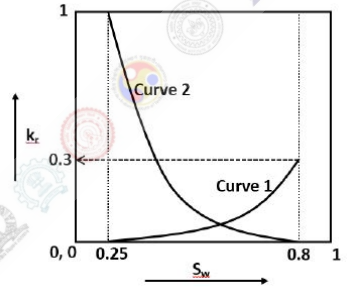
\includegraphics[width=0.5\textwidth]{figures/29.png}
\end{center}
\vspace{0.5cm}

% Question 30
\questionb{An oil reservoir of 1000 m\(^2\) area and thickness of 10 m has a porosity of 30\%. The climate water saturation is 20\%. Initial formation volume factor \(B_{of} = 1.2 \quad \text{reservoir m}^3\). Assuming average oil flow rate of 2 m\(^3\)/day (at surface condition), the life of reservoir is \_\_\_\_\_ days.}{30}
\vspace{0.5cm}

\questionb{A self-flowing production well of depth \(3,000 \, \text{m}\) having oil with density \(850 \, \text{kg/m}^3\) is shut-in for workover job. The shut-in pressure at the surface is \(70 \times 10^5 \, \text{N/m}^2\). The density of the mud required to kill the well will be \_\_\_\_\_ kg/m\(^3\). (\(g = 9.81 \, \text{m/s}^2\), write answer with one decimal place)}{31}
\vspace{0.5cm}

% Question 32
\questionb{In a directional well, the kick off point has a true vertical depth (TVD) of \(1000 \, \text{m}\) and the end of buildup section has a TVD of \(1200 \, \text{m}\). The buildup section for directional drilling has a horizontal displacement of \(200 \, \text{m}\), after which the tangent section has inclination of \(45^\circ\). A driller monitors the well from the surface location of the well and sees that the target has horizontal departure of \(1000 \, \text{m}\). The TVD of the deepest point of the well is \_\_\_\_\_ meters.}{32}
\vspace{0.5cm}

% Question 33
\questionb{The figure below shows the pressure measured in a well at different depths. AB is gas cap, B is gas oil contact and C is water-oil contact. Density of gas in gas cap is \(2 \, \text{kg/m}^3\), oil density is \(800 \, \text{kg/m}^3\) and water density is \(1000 \, \text{kg/m}^3\). The difference between pressure at point D and point B (\(\text{P}_D - \text{P}_B\)) is \_\_\_\_\_ \(\times 10^5 \, \text{N/m}^2\). (use \(g = 9.81 \, \text{m/s}^2\), write answer with one decimal place)}{33}
\begin{center}
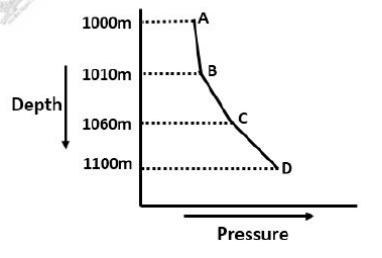
\includegraphics[width=0.5\textwidth]{figures/33.png}
\end{center}
\vspace{0.5cm}

% Question 34
\questionb{A laboratory air-brine capillary pressure of \(1.20 \times 10^5 \, \text{N/m}^2\) has been measured in a reservoir core sample at residual water saturation. The air-brine surface tension is 0.070 N/m, and the brine-oil interfacial tension for the reservoir fluid is 0.025 N/m. The density values of brine and oil are 1080 kg/m\(^3\) and 780 kg/m\(^3\), respectively. Take \(g = 9.81 \, \text{m/s}^2\), and assume identical wetting preferences for the core sample and reservoir. The height of the water-oil transition zone (up to the point of reservoir where connate water saturation is reached) from the free water level is \_\_\_\_\_ meters. (write answer with two decimal places)}{34}
\vspace{0.5cm}

% Question 35
\questionb{The eigenvalues for the matrix 
\[\begin{bmatrix}
1 & 3 \\
4 & 2
\end{bmatrix}\]
are:}{35}
\begin{enumerate}
    \item[(A)] 2 and 5
    \item[(B)] -2 and -5
    \item[(C)] -2 and 5
    \item[(D)] none of the above
\end{enumerate}
\vspace{0.5cm}

\questionb{The temperature time profile for a system is given as follows:
\[\frac{dT}{dt} + 5T = 500,\]
where \(T\) is temperature in °C, and \(t\) is time in hours. The initial conditions are \(T(0) = 500^\circ C\). The temperature of the system after 1 hour is \_\_\_\_\_ °C. (write answer with two decimal places)}{36}
\vspace{0.5cm}

% Question 37
\questionb{A porous medium is blended with three types of sediment fractions, fine pebble gravel with porosity (\(\phi_{pebble} = 38\%\)), sand (\(\phi_{sand} = 32\%\)) and fine sand (\(\phi_{fine\_sand} = 30\%\)). The three sediments are mixed in such proportions that the sand fills the pore volume of fine pebbles completely, and the fine sand fills the pore volume of sand completely. The total porosity of such an irregular system is \_\_\_\_\_ \%. (write answer with two decimal places)}{37}
\vspace{0.5cm}

% Question 38
\questionb{Match the following:}{38}
\begin{enumerate}
    \item[(P)] Sandstone
    \item[(Q)] Limestone
    \item[(R)] Shale
    \item[(S)] Gypsum
    \item[(A)] P-I, Q-I, R-II, S-II
    \item[(B)] P-II,Q-II, R-I, S-I
    \item[(C)] P-I, Q-II, R-I, S-II
    \item[(D)] P-II, Q-I, R-II, S-I
    \item[(I)] Plastic rocks
    \item[(II)] Nonelastic rocks
\end{enumerate}
\vspace{0.5cm}

% Question 39
\questionb{Oil of density 900 kg/m\(^3\) is flowing at 100 m\(^3\)/day through a horizontal pipeline having a diameter reduction from 0.1 m to 0.05 m as shown in the following figure. The kinetic energy pressure drop (P\(_1\) - P\(_2\)) caused by the diameter change is \_\_\_\_\_ N/m\(^2\). (Assume frictional losses to be negligible, write answer with one decimal place)}{39}
\begin{center}
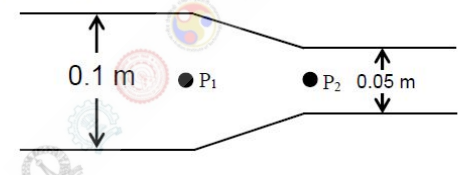
\includegraphics[width=0.5\textwidth]{figures/39.png}
\end{center}
\vspace{0.5cm}

% Question 40
\questionb{Match the following EOR techniques and the principle behind them:}{40}
\begin{enumerate}
    \item[(P)] Surfactant flooding
    \item[(Q)] Polymer flooding
    \item[(R)] Steam flooding
    \item[(S)] Sea water flooding
    \item[(I)] Lower the viscosity of the oil phase
    \item[(II)] Increase the viscosity of the aqueous phase
    \item[(III)] Lower the oil-water interfacial tension
    \item[(IV)] Influence the wettability of the rock
    \item[(A)] P-I, Q-II, R-III, S-IV
    \item[(B)] P-II, Q-III, R-IV, S-I
    \item[(C)] P-III, Q-II, R-I, S-IV
    \item[(D)] P-III, Q-I, R-II, S-IV
\end{enumerate}
\vspace{0.5cm}

\questionb{The viscosity - shear rate curve for a fluid is shown in the following plot. Which one of the following options best describes the behavior of the fluid in the regions I, II, and III, respectively?}{41}
\begin{center}
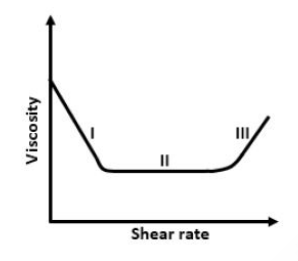
\includegraphics[width=0.5\textwidth]{figures/41.png}
\end{center}
\begin{enumerate}
    \item[(A)] Newtonian, Shear thinning, Shear thickening
    \item[(B)] Shear thinning, Newtonian, Shear thickening
    \item[(C)] Shear thickening, Newtonian, Shear thinning
    \item[(D)] Shear thinning, Shear thickening, Newtonian
\end{enumerate}
\vspace{0.5cm}

% Question 42
\questionb{The value of constant \( a \) for which:
\[f(x) = 
\begin{cases} 
ax^2, & 0 \leq x \leq 5 \\ 
0, & \text{otherwise}
\end{cases}\]
is a valid probability density function, is (given, \( a \geq 0 \)):}{42}
\begin{enumerate}
    \item[(A)] \(\frac{1}{125}\)
    \item[(B)] \(\frac{3}{125}\)
    \item[(C)] \(\frac{6}{125}\)
    \item[(D)] \(\frac{9}{125}\)
\end{enumerate}
\vspace{0.5cm}

% Question 43
\questionb{\[z = \frac{3i^{30} - i^{19}}{2i - 1}, \quad \text{where} \quad i = \sqrt{-1}, \quad \text{would simplify to:}\]}{43}
\begin{enumerate}
    \item[(A)] \( 1 - i \)
    \item[(B)] 1
    \item[(C)] \(-i\)
    \item[(D)] \( 1 + i\)
\end{enumerate}
\vspace{0.5cm}

% Question 44
\questionb{A well of radius 0.25 m is drilled. Mud invasion in the formation caused a skin radius of 2 m and reduced the permeability of the damaged zone to 30 mD. Well test revealed that the skin factor of the damaged zone is 2.3. The permeability of the unaffected formation will be \_\_\_\_\_ mD. (write answer with one decimal place)}{44}
\vspace{0.5cm}

% Question 45
\questionb{The average reservoir pressure and fracture gradient of petroleum formation at a depth of 4,000 m are 30,000 kN/m\(^2\) and 16 (kN/m\(^2\))m, respectively. The density of the formation is 2290 kg/m\(^3\). If the reservoir pressure declines to 20,000 kN/m\(^2\) after a few years of production, the fracture gradient of the formation is \_\_\_\_\_ (kN/m\(^2\))m. (write answer with one decimal place)}{45}
\vspace{0.5cm}

\questionb{Match the following:}{46}
\begin{enumerate}
    \item[(P)] Gamma ray log
    \item[(Q)] Resistivity log
    \item[(R)] Cement bond log
    \item[(S)] NMR log
    \item[(I)] Water saturation
    \item[(II)] Acoustic waves
    \item[(III)] Permeability
    \item[(IV)] Lithology
    \item[(A)] P-IV, Q-I, R-II, S-III
    
    \item[(B)] P-I, Q-II, R-III, S-IV
    \item[(C)] P-I, Q-III, R-II, S-IV
    \item[(D)] P-IV, Q-II, R-I, S-III
\end{enumerate}
\vspace{0.5cm}

% Question 47
\questionb{The sonic log travel time in a loosely consolidated formation is 260 µs/m. The matrix and fluid travel times are 130 µs/m and 618 µs/m, respectively. A correction factor of 1.0 may be used in a Wyllie time average equation for simplification. The calculated formation porosity using the Wyllie time average equation is \_\_\_\_\_ \%. (write answer with two decimal places)}{47}
\vspace{0.5cm}

% Question 48
\questionb{An oil emulsion having 15\% water cut by weight is being treated in a horizontal heater-treater unit at the rate of 6000 kg/hr. The inlet temperature of the emulsion is \( 30^\circ C \) and operating temperature of the heater-treater is \( 40^\circ C \). The specific heat capacity of water and oil are 1 kcal/kg\( ^\circ C \) and 0.5 kcal/kg\( ^\circ C \), respectively. Assuming 10\% of the total heat input is lost to the surroundings, the total heat energy required to break the emulsion in the heater-treater unit is \_\_\_\_\_ kcal/hr. (write answer with one decimal place)}{48}
\vspace{0.5cm}

% Question 49
\questionb{An oil well has a flowing bottom hole pressure of 3000 psi and the reservoir has an average pressure of 3250 psi. A pressure build-up test reveals that the slope of the straight line portion of Horner's plot is 38.5 psi/cycle and skin factor of the well is 3. The flow efficiency of this well is \_\_\_\_\_. (write answer with two decimal places)}{49}
\vspace{0.5cm}

% Question 50
\questionb{A pressure charged, casing pressure operated gas lift valve is installed at a depth of 200 m and the bellow pressure of this valve is \( 50 \times 10^5 \, \text{N/m}^2 \) under operating conditions. The tubing pressure is \( 30 \times 10^5 \, \text{N/m}^2 \) at the valve depth. The area of the bellow and the port are 6 and 0.6 cm\( ^2 \), respectively. The opening pressure of the gas lift valve under operating condition is \_\_\_\_\_ \( \times 10^5 \, \text{N/m}^2 \). (write answer with one decimal place)}{50}
\vspace{0.5cm}

% Question 51
\questionb{Match the following:}{51}
\begin{enumerate}
    \item[(P)] Coal bed methane
    \item[(Q)] Tight gas
    \item[(R)] Gas hydrate
    \item[(S)] Associated gas
    \item[(I)] Requires natural or artificial fractures
    \item[(II)] Exists in solid phase
    \item[(III)] Gas adsorbed on surface in micro-pores
    \item[(IV)] Dissolved in crude oil
    \item[(A)] P-I, Q-II, R-III, S- IV
    \item[(B)] P-IV, Q-III, R-I, S- II
    \item[(C)] P- III, Q-I, R-II, S- IV
    \item[(D)] P-IV, Q-I, R-II, S-III
\end{enumerate}
\vspace{0.5cm}

% Question 52
\questionb{Match the following, in the context of treatment of oil spills:}{52}
\begin{enumerate}
    \item[(P)] Boom
    \item[(Q)] Adsorbent
    \item[(R)] Skimmer
    \item[(S)] Biostimulation
    \item[(I)] Use of chemical fertilizers to enhance the rate of oil degradation by microbes
    \item[(II)] Mechanized equipment for removing floating oil from water surface
    \item[(III)] Floating physical barrier to divert oil to a recovery area
    \item[(IV)] Oleophilic material to attract oil, which can be removed subsequently
    \item[(A)] P - I, Q - IV, R - II, S - III
    \item[(B)] P - III, Q - IV, R - II, S - I
    \item[(C)] P - III, Q - II, R - IV, S - I
    \item[(D)] P - I, Q - III, R - IV, S - II
\end{enumerate}
\vspace{0.5cm}

% Question 53
\questionb{Match the following:}{53}
\begin{enumerate}
    \item[(P)] Aquifer
    \item[(Q)] Aquitard
    \item[(R)] Aquichudes
    
    \item[(I)] Slows down the movement of water and not good for water (or CO\(_2\)) injection
    \item[(II)] Evaporite rocks, such as halides or anhydrite, retarding upward movement of water/CO\(_2\)
    \item[(III)] Preferentially stores CO\(_2\) but not water
    \item[(IV)] Rocks with sufficient permeability to conduct water, into which water (or CO\(_2\)) may be injected
    \item[(A)] P - I, Q - III, R - IV
    \item[(B)] P - IV, Q - I, R - III
    \item[(C)] P - IV, Q - I, R - II
    \item[(D)] P - IV, Q - II, R - III
\end{enumerate}
\vspace{0.5cm}

% Question 54
\questionb{Synthetic Aperture Radar (SAR), used for oil spill monitoring and detection, is based on the:
\begin{enumerate}
    \item [(A)] dampening effect oil has on capillary and short ocean surface waves, as seen in the radar backscatter signal.
    \item [(B)] radar backscatter signal only from navigating ships.
    \item [(C)] frequency change in the radar backscatter signal from flights over the sea.
    \item [(D)] physical sample collection from random locations on the high seas.
\end{enumerate}
}{54}
\vspace{0.5cm}

% Question 55
\questionb{The below figure shows the phase diagram of free methane gas and methane hydrate for a pure water and pure methane system. Match the zones marked (I), (II), (III) and (IV) with different state of phases listed below.
\begin{center}
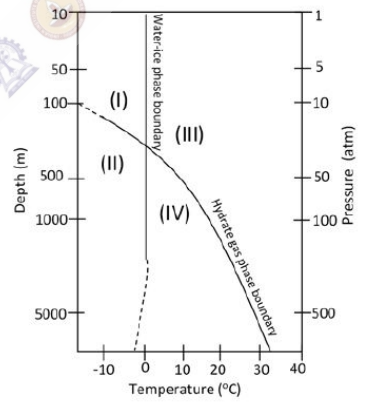
\includegraphics[width=0.5\textwidth]{figures/55.png}
\end{center}
\begin{enumerate}
    \item [(P)] Methane hydrate + water + gas
    \item [(Q)]Methane gas + water
    \item [(R)]Methane gas + ice
    \item [(S)]Methane hydrate + ice + gas
\end{enumerate}}{55}
\begin{enumerate}
    \item [(A)] I-R, II-S, III-P, IV-Q
    \item [(B)]I-R, II-Q, III-P, IV-S
    \item [(C)]I-R, II-S, III-Q, IV-P
    \item [(D)]I-R, II-P, III-S, IV-Q
\end{enumerate}
\vspace{0.5cm}

\begin{center}
\textbf{END OF QUESTION PAPER}
\rule{\textwidth}{0.5pt} 
\end{center}

\end{document}